\def\paperversiondraft{draft}
\def\paperversionblind{blind}
\def\paperversioncamera{camera}

% If no special paper-version is requested, compile in draft mode
\ifx\paperversion\paperversionblind
\else
  \ifx\paperversion\paperversioncamera
  \else
     \def\paperversion{draft}
  \fi
\fi

\def\grammarlyon{on}

\ifx\grammarly\grammarlyon
\def\review{}
\else
\def\review{review,}
\fi

\ifx\paperversion\paperversiondraft
  \documentclass[sigplan,\review anonymous]{acmart}
\fi

\ifx\paperversion\paperversionblind
  \documentclass[sigplan,\review anonymous]{acmart}
\fi

\ifx\paperversion\paperversioncamera
  \documentclass[sigplan]{acmart}\settopmatter{}
\fi

\usepackage{colortbl}

% 'draftonly' environment
\usepackage{environ}
\ifx\paperversion\paperversiondraft
\newenvironment{draftonly}{}{}
\else
\NewEnviron{draftonly}{}
\fi

% Most PL conferences are edited by conference-publishing.com. Follow their
% advice to add the following packages.
%
% The first enables the use of UTF-8 as character encoding, which is the
% standard nowadays. The second ensures the use of font encodings that support
% accented characters etc. (Why should I use this?). The mictotype package
% enables certain features 'to­wards ty­po­graph­i­cal per­fec­tion
\usepackage[utf8]{inputenc}
\usepackage[T1]{fontenc}
\usepackage{microtype}

\usepackage{xargs}
\usepackage{lipsum}
\usepackage[textsize=tiny]{todonotes}
\usepackage{xparse}
\usepackage{xifthen, xstring}
\usepackage[normalem]{ulem}
\usepackage{xspace}
\usepackage{marginnote}
\makeatletter
\font\uwavefont=lasyb10 scaled 652

\newcommand\colorwave[1][blue]{\bgroup\markoverwith{\lower3\p@\hbox{\uwavefont\textcolor{#1}{\char58}}}\ULon}
\makeatother

\ifx\paperversion\paperversiondraft
\newcommand\createtodoauthor[2]{%
\def\tmpdefault{emptystring}
\expandafter\newcommand\csname #1\endcsname[2][\tmpdefault]{\def\tmp{##1}\ifthenelse{\equal{\tmp}{\tmpdefault}}
   {\todo[linecolor=#2,backgroundcolor=#2,bordercolor=#2]{\textbf{#1:} ##2}}
   {\ifthenelse{\equal{##2}{}}{\colorwave[#2]{##1}\xspace}{\todo[linecolor=#2,backgroundcolor=#2,bordercolor=#2]{\textbf{#1:} ##2}\colorwave[#2]{##1}}}}
\expandafter\newcommand\csname #1f\endcsname[2][\tmpdefault]{
	\smash{\marginnote{
		\todo[inline,linecolor=#2,backgroundcolor=#2,bordercolor=#2]{\textbf{#1 (Figure):} ##2}}}
   }
}
%
\else
\newcommand\createtodoauthor[2]{%
\def\tmpdefault{emptystring}%
\expandafter\newcommand\csname #1\endcsname[2][\tmpdefault]{}%
\expandafter\newcommand\csname #1f\endcsname[2][\tmpdefault]{}%
}%
\fi

% Broaden margins to make room for todo notes
\makeatletter
\patchcmd{\@addmarginpar}{\ifodd\c@page}{\ifodd\c@page\@tempcnta\m@ne}{}{}
\makeatother
\ifx\paperversion\paperversiondraft
  \makeatletter
  \if@ACM@journal
    \geometry{asymmetric}
    \paperwidth=\dimexpr \paperwidth + 3.5cm\relax
    \oddsidemargin=\dimexpr\oddsidemargin + 0cm\relax
    \evensidemargin=\dimexpr\evensidemargin + 0cm\relax
    \marginparwidth=\dimexpr \marginparwidth + 3cm\relax
    \setlength{\marginparwidth}{4.6cm}
    % This makeatletter box helps to move notes to the right
    \makeatletter
    \long\def\@mn@@@marginnote[#1]#2[#3]{%
      \begingroup
        \ifmmode\mn@strut\let\@tempa\mn@vadjust\else
          \if@inlabel\leavevmode\fi
          \ifhmode\mn@strut\let\@tempa\mn@vadjust\else\let\@tempa\mn@vlap\fi
        \fi
        \@tempa{%
          \vbox to\z@{%
            \vss
            \@mn@margintest
            \if@reversemargin\if@tempswa
                \@tempswafalse
              \else
                \@tempswatrue
            \fi\fi
            %\if@tempswa
              \rlap{%
                \if@mn@verbose
                  \PackageInfo{marginnote}{xpos seems to be \@mn@currxpos}%
                \fi
                \begingroup
                  \ifx\@mn@currxpos\relax\else\ifx\@mn@currxpos\@empty\else
                      \kern-\dimexpr\@mn@currxpos\relax
                  \fi\fi
                  \ifx\@mn@currpage\relax
                    \let\@mn@currpage\@ne
                  \fi
                  \if@twoside\ifodd\@mn@currpage\relax
                      \kern\oddsidemargin
                    \else
                      \kern\evensidemargin
                    \fi
                  \else
                    \kern\oddsidemargin
                  \fi
                  \kern 1in
                \endgroup
                \kern\marginnotetextwidth\kern\marginparsep
                \vbox to\z@{\kern\marginnotevadjust\kern #3
                  \vbox to\z@{%
                    \hsize\marginparwidth
                    \linewidth\hsize
                    \kern-\parskip
                    \marginfont\raggedrightmarginnote\strut\hspace{\z@}%
                    \ignorespaces#2\endgraf
                    \vss}%
                  \vss}%
              }%
          }%
        }%
      \endgroup
    }
    \makeatother
  \else
    \paperwidth=\dimexpr \paperwidth + 6cm\relax
    \oddsidemargin=\dimexpr\oddsidemargin + 3cm\relax
    \evensidemargin=\dimexpr\evensidemargin + 3cm\relax
    \marginparwidth=\dimexpr \marginparwidth + 3cm\relax
    \setlength{\marginparwidth}{4.6cm}
  \fi
  \makeatother
\fi

% We use the following color scheme
% 
% This scheme is both print-friendly and colorblind safe for
% up to four colors (including the red tones makes it not
% colorblind safe any more)
%
% https://colorbrewer2.org/#type=qualitative&scheme=Paired&n=4

\definecolor{pairedNegOneLightGray}{HTML}{cacaca}
\definecolor{pairedNegTwoDarkGray}{HTML}{827b7b}
\definecolor{pairedOneLightBlue}{HTML}{a6cee3}
\definecolor{pairedTwoDarkBlue}{HTML}{1f78b4}
\definecolor{pairedThreeLightGreen}{HTML}{b2df8a}
\definecolor{pairedFourDarkGreen}{HTML}{33a02c}
\definecolor{pairedFiveLightRed}{HTML}{fb9a99}
\definecolor{pairedSixDarkRed}{HTML}{e31a1c}

\createtodoauthor{grosser}{pairedOneLightBlue}
\createtodoauthor{authorTwo}{pairedTwoDarkBlue}
\createtodoauthor{authorThree}{pairedThreeLightGreen}
\createtodoauthor{authorFour}{pairedFourDarkGreen}
\createtodoauthor{authorFive}{pairedFiveLightRed}
\createtodoauthor{authorSix}{pairedSixDarkRed}

\graphicspath{{./images/}}

% Define macros that are used in this paper
%
% We require all macros to end with a delimiter (by default {}) to enusure
% that LaTeX adds whitespace correctly.
\makeatletter
\newcommand\requiredelimiter[2][########]{%
  \ifdefined#2%
    \def\@temp{\def#2#1}%
    \expandafter\@temp\expandafter{#2}%
  \else
    \@latex@error{\noexpand#2undefined}\@ehc
  \fi
}
\@onlypreamble\requiredelimiter
\makeatother

\newcommand\newdelimitedcommand[2]{
\expandafter\newcommand\csname #1\endcsname{#2}
\expandafter\requiredelimiter
\csname #1 \endcsname
}

\newdelimitedcommand{toolname}{Tool}


% Print \autoref as "Section X.Y.Z"
\renewcommand*{\sectionautorefname}{Section}
\renewcommand*{\subsectionautorefname}{Section}
\renewcommand*{\subsubsectionautorefname}{Section}

% \circled command to print a colored circle.
% \circled{1} pretty-prints "(1)"
% This is useful to refer to labels that are embedded within figures.
\usepackage{tikz}
\usetikzlibrary{arrows}
\usetikzlibrary{shapes}
\newcommand*\circled[1]{\tikz[baseline=(char.base)]{
            \node[shape=circle,fill=pairedOneLightBlue,inner sep=1pt] (char) {#1};}}


%% Note: Authors migrating a paper from traditional SIGPLAN
%% proceedings format to PACMPL format should change 'sigplan' to
%% 'acmsmall'.


%% Some recommended packages.
\usepackage{booktabs}   %% For formal tables:
                        %% http://ctan.org/pkg/booktabs
\usepackage{subcaption} %% For complex figures with subfigures/subcaptions
                        %% http://ctan.org/pkg/subcaption


\makeatletter\if@ACM@journal\makeatother
%% Journal information (used by PACMPL format)
%% Supplied to authors by publisher for camera-ready submission
\acmJournal{PACMPL}
\acmVolume{1}
\acmNumber{1}
\acmArticle{1}
\acmYear{2017}
\acmMonth{1}
\acmDOI{10.1145/nnnnnnn.nnnnnnn}
\startPage{1}
\else\makeatother
%% Conference information (used by SIGPLAN proceedings format)
%% Supplied to authors by publisher for camera-ready submission
\acmConference[PL'17]{ACM SIGPLAN Conference on Programming Languages}{January 01--03, 2017}{New York, NY, USA}
\acmYear{2017}
\acmISBN{978-x-xxxx-xxxx-x/YY/MM}
\acmDOI{10.1145/nnnnnnn.nnnnnnn}
\startPage{1}
\fi


%% Copyright information
%% Supplied to authors (based on authors' rights management selection;
%% see authors.acm.org) by publisher for camera-ready submission
\setcopyright{none}             %% For review submission
%\setcopyright{acmcopyright}
%\setcopyright{acmlicensed}
%\setcopyright{rightsretained}
%\copyrightyear{2017}           %% If different from \acmYear


%% Bibliography style
\bibliographystyle{ACM-Reference-Format}
%% Citation style
%% Note: author/year citations are required for papers published as an
%% issue of PACMPL.
%\citestyle{acmauthoryear}  %% For author/year citations
%\citestyle{acmnumeric}     %% For numeric citations
%\setcitestyle{nosort}      %% With 'acmnumeric', to disable automatic
                            %% sorting of references within a single citation;
                            %% e.g., \cite{Smith99,Carpenter05,Baker12}
                            %% rendered as [14,5,2] rather than [2,5,14].
%\setcitesyle{nocompress}   %% With 'acmnumeric', to disable automatic
                            %% compression of sequential references within a
                            %% single citation;
                            %% e.g., \cite{Baker12,Baker14,Baker16}
                            %% rendered as [2,3,4] rather than [2-4].



\begin{document}

%% Title information
\title[Short Title]{Full Title}         %% [Short Title] is optional;
                                        %% when present, will be used in
                                        %% header instead of Full Title.
\subtitle{Subtitle}                     %% \subtitle is optional


%% Author information
%% Contents and number of authors suppressed with 'anonymous'.
%% Each author should be introduced by \author, followed by
%% \authornote (optional), \orcid (optional), \affiliation, and
%% \email.
%% An author may have multiple affiliations and/or emails; repeat the
%% appropriate command.
%% Many elements are not rendered, but should be provided for metadata
%% extraction tools.

%% Author with single affiliation.
\author{First1 Last1}
\authornote{with author1 note}          %% \authornote is optional;
                                        %% can be repeated if necessary
\orcid{nnnn-nnnn-nnnn-nnnn}             %% \orcid is optional
\affiliation{
  \position{Position1}
  \department{Department1}              %% \department is recommended
  \institution{Institution1}            %% \institution is required
  \streetaddress{Street1 Address1}
  \city{City1}
  \state{State1}
  \postcode{Post-Code1}
  \country{Country1}
}
\email{first1.last1@inst1.edu}          %% \email is recommended

%% Author with two affiliations and emails.
\author{First2 Last2}
\authornote{with author2 note}          %% \authornote is optional;
                                        %% can be repeated if necessary
\orcid{nnnn-nnnn-nnnn-nnnn}             %% \orcid is optional
\affiliation{
  \position{Position2a}
  \department{Department2a}             %% \department is recommended
  \institution{Institution2a}           %% \institution is required
  \streetaddress{Street2a Address2a}
  \city{City2a}
  \state{State2a}
  \postcode{Post-Code2a}
  \country{Country2a}
}
\email{first2.last2@inst2a.com}         %% \email is recommended
\affiliation{
  \position{Position2b}
  \department{Department2b}             %% \department is recommended
  \institution{Institution2b}           %% \institution is required
  \streetaddress{Street3b Address2b}
  \city{City2b}
  \state{State2b}
  \postcode{Post-Code2b}
  \country{Country2b}
}
\email{first2.last2@inst2b.org}         %% \email is recommended

\begin{abstract}
% An abstract should consist of six main sentences:
%  1. Introduction. In one sentence, what’s the topic?
%  2. State the problem you tackle.
%  3. Summarize (in one sentence) why nobody else has adequately answered the research question yet.
%  4. Explain, in one sentence, how you tackled the research question.
%  5. In one sentence, how did you go about doing the research that follows from your big idea.
%  6. As a single sentence, what’s the key impact of your research?

% (http://www.easterbrook.ca/steve/2010/01/how-to-write-a-scientific-abstract-in-six-easy-steps/)
\lipsum[1]
\end{abstract}


% Only add ACM notes and keywords in camera ready version
% Drop citations and footnotes in draft and blind mode.
\ifx\paperversion\paperversioncamera
%% 2012 ACM Computing Classification System (CSS) concepts
%% Generate at 'http://dl.acm.org/ccs/ccs.cfm'.
\begin{CCSXML}
<ccs2012>
<concept>
<concept_id>10011007.10011006.10011008</concept_id>
<concept_desc>Software and its engineering~General programming languages</concept_desc>
<concept_significance>500</concept_significance>
</concept>
<concept>
<concept_id>10003456.10003457.10003521.10003525</concept_id>
<concept_desc>Social and professional topics~History of programming languages</concept_desc>
<concept_significance>300</concept_significance>
</concept>
</ccs2012>
\end{CCSXML}

\ccsdesc[500]{Software and its engineering~General programming languages}
\ccsdesc[300]{Social and professional topics~History of programming languages}
%% End of generated code


%% Keywords
%% comma separated list
\keywords{keyword1, keyword2, keyword3}  %% \keywords is optional

\else
\settopmatter{printacmref=false} % Removes citation information below abstract
\renewcommand\footnotetextcopyrightpermission[1]{} % removes footnote with conference information in first column
\fi

%% \maketitle
%% Note: \maketitle command must come after title commands, author
%% commands, abstract environment, Computing Classification System
%% environment and commands, and keywords command.
\maketitle
\ifx\grammarly\grammarlyon 
\onecolumn 
\else 
\fi

\section{Introduction}

Of this super cool article \ldots
\grosser{A simple comment refering to a particular location}

If there is \authorTwo[some text we want to refer to specifically]{this looks
particularly interesting} we can refer to this text from within our comments.

And here we only underline \authorTwo[Text]{} that is interesting, but do not
actually comment.

Now we have a sequence of comments,
\authorThree{Comment 3}
\authorFour{Comment 4}
\authorFive{Comment 5}
\authorSix{Comment 6}
which should not introduce overlong white space sequences.

Sometimes it is also important to \emph{emphasize} text to understand if it is
underlined or printed in italic.

We sometimes use macros to state that a tool as the name \toolname{} in a
flexible way.

\lipsum[1-3]

\begin{figure}
% Link to figure
%
% https://docs.google.com/drawings/d/1juKp43D3rLC-luBQPwQZ_wCnDK2S_6C1k6USV0wKE0g/edit?usp=sharing
\includegraphics[width=\columnwidth]{overview.pdf}
\caption{Our key idea visualized}
\grosserf{Replace this figure with your own drawing.}
\end{figure}

~\\
Our contributions are:
\grosser{Always state your contributions explicitly: (A) this makes it
easy for the reader to understand what novelty is presented, and (B)
these contributions help you to focus. In particular, the objective of
the remaining paper should be to support the claims stated here.
}
\begin{itemize}
	\item Contribution 1
	\item Contribution 2
	\item Contribution 3
	\item Contribution 4
\end{itemize}

\section{Our New Idea}

\lipsum[1-3]

\section{Implementation}

\section{Related Work}

\lipsum[1-3]

\grosser{Related work should always be at the end of the document,
         as it otherwise becomes an obstacle your reader must
	 overcome before reaching your idea. For details see:
	 \url{https://www.microsoft.com/en-us/research/academic-program/write-great-research-paper/}
}

\section{Conclusion}
\lipsum[1]


%% Acknowledgments
\begin{acks}                            %% acks environment is optional
                                        %% contents suppressed with 'anonymous'
  %% Commands \grantsponsor{<sponsorID>}{<name>}{<url>} and
  %% \grantnum[<url>]{<sponsorID>}{<number>} should be used to
  %% acknowledge financial support and will be used by metadata
  %% extraction tools.
  This material is based upon work supported by the
  \grantsponsor{GS100000001}{National Science
    Foundation}{http://dx.doi.org/10.13039/100000001} under Grant
  No.~\grantnum{GS100000001}{nnnnnnn} and Grant
  No.~\grantnum{GS100000001}{mmmmmmm}.  Any opinions, findings, and
  conclusions or recommendations expressed in this material are those
  of the author and do not necessarily reflect the views of the
  National Science Foundation.
\end{acks}

%% Bibliography
%\bibliography{bibfile}


%% Appendix
\newpage
\appendix
\begin{draftonly}
\section{Formatting Guidelines}

These formatting guidelines aim to standartize our writing. They ensure that
papers with multiple authors have a consistent look and that commonly occuring
items are formatted in ways that are known to work well.

\subsection{Figures}

\paragraph{Color Scheme} 

In Figures we use a color scheme that is print-friendly and also visible
with red-green blindness. The following colors are all print-friendly
and red-green save when only using Color 1-4:

\medskip
{
	\small
\newcolumntype{a}{>{\columncolor{pairedOneLightBlue}}c}
\newcolumntype{b}{>{\columncolor{pairedTwoDarkBlue}}c}
\newcolumntype{d}{>{\columncolor{pairedThreeLightGreen}}c}
\newcolumntype{e}{>{\columncolor{pairedFourDarkGreen}}c}
\newcolumntype{f}{>{\columncolor{pairedFiveLightRed}}c}
\newcolumntype{g}{>{\columncolor{pairedSixDarkRed}}c}

\begin{tabular}{a b d e f g}
Color 1 & Color 2 & Color 3 & Color 4 & Color 5 & Color 6\\
\#a6cee3 & \#1f78b4 & \#b2df8a & \#33a02c & \#fb9a99 & \#e31a1c
\end{tabular}
}

We de-emphasize components in figures by using additionally two shades of gray.
Especially in complex figures, it is often helpful to de-emphasize visual
elements that we want to represent but that should not be the focus of a
reader's attention.

\medskip
{
	\small
\newcolumntype{h}{>{\columncolor{pairedNegOneLightGray}}c}
\newcolumntype{i}{>{\columncolor{pairedNegTwoDarkGray}}c}

\begin{tabular}{h i}
Color -1 & Color -2\\
\#cacaca & \#827b7b\\
\end{tabular}
}

Single-color graphs are plotted in Color 1 - Light Blue.

\paragraph{Labels in Figures}
Complex diagrams often benefit from labels inside the diagrams. We suggest to
use a filled circle (e.g, in light blue) to highlight these numbers and use
these references, e.g., \circled{1} implemented as \texttt{\textbackslash{}circled\{1\}}, in the text to refer to them.

\subsubsection{Plots} We use matplotlib to create performance
plots such as \autoref{fig:speedup}. We use the following
formatting guidelines:
\begin{itemize}
  \item Use a vertical y-label to make it easier to read.
  \item Remove top and right frames to reduce visual noise
	and allow the reader to focus on the data in the
	figure.
  \item Provide the concrete data at the top of each bar.
\end{itemize}

\noindent
We also suggest to follow these technical remarks:
\begin{itemize}
  \item Create pdf plots and do not use bitmap formats (e.g., png) to
	ensure high quality when zooming in.
  \item Avoid Type-3 bitmap fonts by
	setting fonttype to 42.
\end{itemize}

\begin{figure}
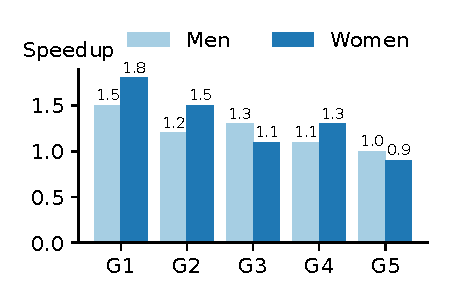
\includegraphics[width=\columnwidth]{plots/speedup}
\caption{Improved running speed after 4 weeks of training.
}
\label{fig:speedup}
\end{figure}

\end{draftonly}


\end{document}
